% =====================================================================
%  Project Report — Natural Language Engineering (NLE) style
%  Receipt / Invoice Information Extraction with Layout-Aware Transformers
%
%  Compiles as-is on Overleaf (pdfLaTeX). It uses the standard `article`
%  class styled to resemble the NLE journal paper. If you have the
%  official nle.cls, replace the \documentclass line with \documentclass{nle}
%  and remove the geometry/titling tweaks below.
% =====================================================================
\documentclass[11pt]{article}

\usepackage[utf8]{inputenc}
\usepackage[T1]{fontenc}
\usepackage{times}
\usepackage[a4paper,margin=1in]{geometry}
\usepackage{amsmath,amssymb}
\usepackage{graphicx}
\usepackage{booktabs}
\usepackage{multirow}
\usepackage{pgfplots}
\pgfplotsset{compat=1.17}
\usepackage{url}
\usepackage[round]{natbib}
\usepackage[hidelinks]{hyperref}
\usepackage{abstract}
\renewcommand{\abstractnamefont}{\normalfont\bfseries}
\renewcommand{\abstracttextfont}{\normalfont\small}

\title{\textbf{Receipt and Invoice Information Extraction with\\
Layout-Aware Transformers}\\[0.4em]
\large How much does 2D layout add over text alone? A field-wise analysis}

\author{
\large Disha Sahu \quad Chandan Giri\\[0.5em]
\normalsize Deep Learning Course Project\\[0.6em]
\small Dataset: ICDAR~2019 SROIE (Task~3)\\[0.3em]
\small Code: \url{https://github.com/Disha-01-alt/field-ai}\\[0.3em]
\small Model: \url{https://huggingface.co/dishasahu/fieldai-layoutlm-sroie}
}
\date{}

\begin{document}
\maketitle

\begin{abstract}
\noindent
Scanned receipts and invoices are \emph{visually rich documents}: their meaning
depends not only on the words they contain but on where those words sit on the
page. We study key information extraction (KIE) from receipts---extracting the
\textsc{company}, \textsc{date} and \textsc{total} fields---and ask a single
focused question: \emph{how much does two-dimensional spatial layout add over
pure text?} We build a three-tier benchmark on the ICDAR~2019 SROIE dataset:
(i)~a deterministic OCR\,+\,regular-expression baseline, (ii)~a text-only
\texttt{BERT} token classifier, and (iii)~\texttt{LayoutLM}, which augments the
same text tokens with 2D bounding-box embeddings. All three systems are decoded
to field strings and scored by one shared evaluation harness, making the
comparison strictly apples-to-apples. LayoutLM reaches a macro-averaged
field F1 of \textbf{91.94\%}, improving over the text-only BERT baseline by
\textbf{+21.41} points. The gain is highly field-dependent: layout contributes
\textbf{+38.43} F1 on \textsc{company} and \textbf{+27.79} on \textsc{total},
but essentially nothing on \textsc{date} ($-2.00$), which is already recoverable
from text. This pattern---large gains where text is spatially ambiguous, none
where it is syntactically self-identifying---is the central empirical finding
of the project. We release the fine-tuned model and an end-to-end image demo.

\medskip
\noindent\textbf{Keywords:} key information extraction, document AI, LayoutLM,
token classification, visually rich documents, SROIE.
\end{abstract}

% =====================================================================
\section{Introduction}
% =====================================================================
Automatically extracting structured fields from scanned receipts and invoices is
a long-standing problem in document understanding, with direct applications in
expense management, accounting automation and auditing. The task is deceptively
hard: real receipts vary in template, font, illumination, skew and OCR quality,
and the same literal string (e.g.\ a currency amount) may appear many times on a
single document in different roles---line item, subtotal, tax, change, or the
grand total we actually want.

Standard natural language processing treats a document as a one-dimensional
sequence of tokens. Receipts, however, are \emph{two-dimensional}: the store name
sits in the header band, the grand total gravitates to the bottom-right, and
key--value pairs align spatially. This motivates \emph{layout-aware} models such
as LayoutLM \citep{xu2020layoutlm}, which inject the 2D position of each token
into a transformer. Our project quantifies exactly what that spatial signal buys.

\paragraph{Contributions.}
\begin{enumerate}
\item A clean three-tier benchmark (rules $\rightarrow$ text-only transformer
$\rightarrow$ layout-aware transformer) on SROIE, all scored by one unified
field-level harness.
\item A field-wise $\Delta$F1 analysis isolating the marginal utility of layout,
showing it is large and concentrated on spatially-anchored fields
(\textsc{company}, \textsc{total}) and negligible on the syntactically-fixed
\textsc{date} field.
\item A reproducible, released artifact: a public fine-tuned LayoutLM model and
an end-to-end \emph{image $\rightarrow$ fields} inference demo.
\end{enumerate}

% =====================================================================
\section{Related Work}
% =====================================================================
Early receipt extraction relied on templates and hand-written rules, which are
brittle across vendors. Neural KIE reframes the task as sequence labelling.
BERT \citep{devlin2019bert} established transformer-based token classification
for text, but ignores geometry. LayoutLM \citep{xu2020layoutlm} pre-trains text
jointly with 2D positional embeddings derived from OCR bounding boxes, and reports
strong results on form and receipt understanding including SROIE
\citep{huang2019sroie}. We deliberately restrict ourselves to the text\,+\,layout
setting of LayoutLM (not raw pixel features), which is precisely the ``text + 2D
position'' configuration our study targets, and use the SROIE benchmark as the
testbed.

% =====================================================================
\section{Problem Formulation}
% =====================================================================
Each receipt is a sequence of OCR word tokens $w_1,\dots,w_n$ with associated
axis-aligned bounding boxes $b_i=(x_0,y_0,x_1,y_1)$. We cast extraction as
\textbf{BIO token classification} over the label set
\[
\{\texttt{O}\}\cup\{\texttt{B-},\texttt{I-}\}\times
\{\textsc{company},\textsc{date},\textsc{total},\textsc{address}\}.
\]
At inference, contiguous \texttt{B-}/\texttt{I-} spans are decoded back into field
strings. The research fields scored are \textsc{company}, \textsc{date} and
\textsc{total}; \textsc{address} is trained but reported separately.

% =====================================================================
\section{Dataset}
% =====================================================================
We use the \textbf{ICDAR~2019 SROIE} (Task~3) benchmark \citep{huang2019sroie},
comprising 626 annotated real-world receipt scans with word-level OCR boxes and
ground-truth field values. We use a frozen 80/20 split: \textbf{500} training and
\textbf{126} test documents. For LayoutLM, 15\% of the training set (75 documents)
is held out for validation and early stopping, leaving 425 for training.

Following \citet{xu2020layoutlm}, every coordinate is normalised to the integer
range $[0,1000]$:
\begin{equation}
x_{\text{norm}}=\left\lfloor \frac{x}{W}\times 1000 \right\rfloor,\qquad
y_{\text{norm}}=\left\lfloor \frac{y}{H}\times 1000 \right\rfloor,
\end{equation}
clamped to $[0,1000]$, with axis alignment $x_0\le x_1,\; y_0\le y_1$ enforced to
remove OCR box inversions.

% =====================================================================
\section{Methods}
% =====================================================================
\subsection{Tier 1 --- OCR + Regular Expressions}
A zero-learning baseline. \textsc{date} is matched with locale-aware patterns
(\texttt{DD/MM/YYYY}, \texttt{YYYY-MM-DD}, month abbreviations); \textsc{total} is
extracted by currency patterns gated on keywords (\texttt{TOTAL},
\texttt{AMOUNT DUE}) while excluding \texttt{SUBTOTAL}/\texttt{CASH}/\texttt{CHANGE};
\textsc{company} uses a top-of-page positional heuristic.

\subsection{Tier 2 --- BERT (text only)}
\texttt{bert-base-uncased} fine-tuned for token classification. Input is the
WordPiece token sequence with 1D positional encodings only---\emph{no} spatial
information---representing modern NLP without document grounding.

\subsection{Tier 3 --- LayoutLM (text + 2D layout)}
\texttt{microsoft/layoutlm-base-uncased} fine-tuned for token classification. Each
token embedding augments the text and 1D-position embeddings with four 2D
coordinate embeddings:
\begin{equation}
E_i = E_{\text{tok}}(w_i) + E_{\text{pos}}(i)
    + E_{x}(x_{0,i}) + E_{y}(y_{0,i}) + E_{x}(x_{1,i}) + E_{y}(y_{1,i}).
\end{equation}
WordPiece sub-tokens inherit their parent word's box; only the first sub-token
carries the label (continuations are masked with $-100$).

\subsection{Unified evaluation}
To keep the comparison fair, \emph{all three} systems are decoded to
$\{\textsc{company},\textsc{date},\textsc{total}\}$ strings and scored by the same
field-level harness: a prediction is a true positive iff it matches the ground
truth under light, field-aware normalisation (currency symbols, date separators,
case/whitespace). We report per-field Precision/Recall/F1 and the macro-average,
plus the layout contribution $\Delta\text{F1}=\text{F1}_{\text{LayoutLM}}-\text{F1}_{\text{BERT}}$.

% =====================================================================
\section{Experimental Setup}
% =====================================================================
Both transformers use AdamW with a linear warmup schedule and a maximum sequence
length of 512. BERT is trained for 5 epochs (batch 8, lr $3{\times}10^{-5}$).
LayoutLM is trained for up to 12 epochs (batch 4, lr $3{\times}10^{-5}$, weight
decay 0.01, warmup ratio 0.10) with early stopping on validation macro F1
(patience 3); the best checkpoint is restored for testing. All runs use seed 42
on a single T4 GPU. Training LayoutLM to convergence takes $\approx$15 minutes.

% =====================================================================
\section{Results}
% =====================================================================
Table~\ref{tab:main} reports field-wise F1 on the 126-receipt test split, and
Figure~\ref{fig:bench} visualises the comparison. LayoutLM is the only model to
clearly surpass the rule-based baseline and improves the macro F1 over text-only
BERT by \textbf{+21.41} points.

\begin{table}[t]
\centering
\caption{Field-wise test F1 (\%) on SROIE Task~3 (126 receipts), all scored by
the same unified harness. $\Delta$F1 is the layout contribution
(LayoutLM~$-$~BERT).}
\label{tab:main}
\begin{tabular}{llcccc}
\toprule
Model & Modality & Company & Date & Total & \textbf{Macro F1}\\
\midrule
OCR + Regex   & Rules (text)          & 46.03 & 96.36 & 40.48 & \textbf{60.95}\\
BERT-base     & 1D text tokens        & 52.63 & 98.41 & 60.56 & \textbf{70.53}\\
LayoutLM-base & Text + 2D boxes       & \textbf{91.06} & 96.41 & \textbf{88.35} & \textbf{91.94}\\
\midrule
$\Delta$F1    & \textit{layout gain}  & \textbf{+38.43} & $-2.00$ & \textbf{+27.79} & \textbf{+21.41}\\
\bottomrule
\end{tabular}
\end{table}

\begin{figure}[t]
\centering
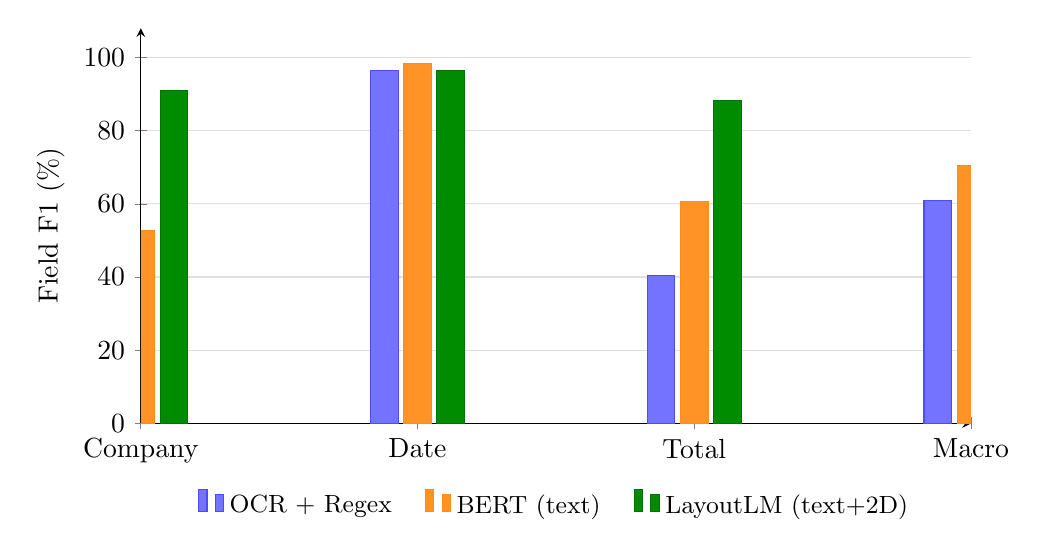
\begin{tikzpicture}
\begin{axis}[
    ybar, bar width=10pt,
    width=\textwidth, height=6.6cm,
    enlarge x limits=0.22,
    ymin=0, ymax=108,
    ytick={0,20,40,60,80,100},
    ylabel={Field F1 (\%)},
    symbolic x coords={Company, Date, Total, Macro},
    xtick=data,
    axis lines=left, ymajorgrids, grid style={gray!25},
    legend style={at={(0.5,-0.15)}, anchor=north, legend columns=3,
                  font=\small, draw=none, /tikz/every even column/.append style={column sep=10pt}},
]
\addplot[fill=blue!55, draw=blue!70] coordinates
  {(Company,46.03) (Date,96.36) (Total,40.48) (Macro,60.95)};
\addplot[fill=orange!85, draw=orange!90] coordinates
  {(Company,52.63) (Date,98.41) (Total,60.56) (Macro,70.53)};
\addplot[fill=green!55!black, draw=green!45!black] coordinates
  {(Company,91.06) (Date,96.41) (Total,88.35) (Macro,91.94)};
\legend{OCR + Regex, BERT (text), LayoutLM (text+2D)}
\end{axis}
\end{tikzpicture}
\caption{Field-wise F1 across the three systems. Layout (green) gives large gains
on \textsc{company} and \textsc{total}, but not on \textsc{date}.}
\label{fig:bench}
\end{figure}

% =====================================================================
\section{Analysis and Discussion}
% =====================================================================
The central question---\emph{how much does layout add over text?}---is answered
decisively, and the field-wise breakdown is more informative than the headline
number.

\paragraph{(1) Company is the largest layout win ($\Delta$F1 $=+38.43$).}
Store names are strongly anchored to the top band of the receipt but are
textually easy to confuse with address lines, tax-invoice titles and category
headers. Text-only BERT manages only 52.63 F1; LayoutLM's vertical-coordinate
embeddings anchor the search to the header region, reaching 91.06. This is the
clearest single piece of evidence that 2D layout resolves ambiguity text cannot.

\paragraph{(2) Grand total benefits strongly ($\Delta$F1 $=+27.79$).}
A receipt contains many monetary values (line items, subtotal, tax, cash, change)
that are textually indistinguishable from the grand total (BERT: 60.56). LayoutLM
learns that the grand total sits in the bottom-right region and reaches 88.35.

\paragraph{(3) Date is the negative control ($\Delta$F1 $=-2.00$).}
Dates follow rigid alphanumeric syntax fully recoverable from text, so both
transformers saturate the field (BERT 98.41, LayoutLM 96.41) and even regex is
near-perfect (96.36). Layout adds no signal; the small negative delta is within
run-to-run noise. This control is what makes the \textsc{company}/\textsc{total}
gains credible: \emph{layout helps precisely where text is ambiguous, and not
where it is not.}

\paragraph{(4) Rules vs.\ learned models.}
The regex baseline is competitive only on \textsc{date} and brittle on
\textsc{company}/\textsc{total}, giving the weakest macro F1 (60.95). BERT improves
with learned patterns (70.53); LayoutLM dominates (91.94) by exploiting the one
signal neither regex nor 1D text can encode: spatial position.

% =====================================================================
\section{Qualitative Evaluation: End-to-End Image Demo}
% =====================================================================
Beyond the benchmark we deploy the full pipeline
\emph{image $\rightarrow$ OCR (Tesseract) $\rightarrow$ LayoutLM
$\rightarrow$ fields} on an unseen, out-of-distribution Indian grocery receipt.
The model correctly recovered \textsc{date} (\texttt{15/05/2024}) and---crucially---%
selected the true grand \textsc{total} (\texttt{325.18}) over the on-receipt
distractors Subtotal (326.00) and Taxable (309.70), exactly the spatial
disambiguation the benchmark measures. It missed \textsc{company}
(``Urban Basket''), an expected \emph{domain-shift} effect: SROIE is dominated by
Malaysian store names with distinct typography, so a novel Indian header style
falls outside the training distribution even though the layout-driven fields
transfer. On in-distribution SROIE receipts the same model scores 91.06 F1 on
\textsc{company}.

% =====================================================================
\section{Limitations and Future Work}
% =====================================================================
(i)~Fine-tuning data is modest (500 receipts) and SROIE-specific, limiting
cross-domain generalisation of region-specific fields such as \textsc{company}.
(ii)~We use LayoutLM-v1 (text + layout) and do not exploit raw pixel features;
LayoutLMv2/v3 with a visual backbone is a natural extension. (iii)~Field matching
uses light normalisation; a stricter character-level protocol could be explored.
Future work includes training on more diverse receipt corpora (e.g.\ CORD) and
adding visual features to close the remaining \textsc{company}/\textsc{address}
gaps.

% =====================================================================
\section{Conclusion}
% =====================================================================
We benchmarked rule-based, text-only and layout-aware extraction on SROIE under a
single unified metric. Two-dimensional layout provides a large and interpretable
benefit---\textbf{+21.41} macro F1 over text alone---concentrated exactly on the
fields whose identity is spatial (\textsc{company}~$+38.43$, \textsc{total}~%
$+27.79$) and absent where text already suffices (\textsc{date}). Layout-aware
transformers are therefore decisively worth their cost for receipt KIE, and our
released model and image demo make the result directly reproducible.

\paragraph{Reproducibility.}
Code: \url{https://github.com/Disha-01-alt/field-ai}. \;
Fine-tuned model: \url{https://huggingface.co/dishasahu/fieldai-layoutlm-sroie}.

% =====================================================================
\begin{thebibliography}{}
\bibitem[Devlin et al.(2019)]{devlin2019bert}
Devlin, J., Chang, M.-W., Lee, K. and Toutanova, K. (2019)
BERT: Pre-training of Deep Bidirectional Transformers for Language Understanding.
In \textit{Proc.\ NAACL-HLT}, pp.~4171--4186.

\bibitem[Huang et al.(2019)]{huang2019sroie}
Huang, Z., Chen, K., He, J., Bai, X., Karatzas, D., Lu, S. and Jawahar, C.~V. (2019)
ICDAR 2019 Competition on Scanned Receipt OCR and Information Extraction (SROIE).
In \textit{Proc.\ ICDAR}, pp.~1516--1520.

\bibitem[Xu et al.(2020)]{xu2020layoutlm}
Xu, Y., Li, M., Cui, L., Huang, S., Wei, F. and Zhou, M. (2020)
LayoutLM: Pre-training of Text and Layout for Document Image Understanding.
In \textit{Proc.\ ACM SIGKDD (KDD)}, pp.~1192--1200.
\end{thebibliography}

\end{document}
